\documentclass[aps,twocolumn,
prl,
%prd,
superscriptaddress,nofootinbib,floatfix]{revtex4-2}



%%%%%%%%%%%%% Packages %%%%%%%%%%%%%

% general
%\usepackage[utf8]{inputenc}
\usepackage{titlesec}

  
% math
\usepackage{mathtools}
\usepackage{amsfonts}
\usepackage{amssymb}
\usepackage{mathrsfs}
\usepackage{bbm}
\usepackage{slashed}
\usepackage{amsmath}
\usepackage{bm}
\usepackage{bbold}


% graphics and colors
\usepackage{graphicx}
\usepackage{color}
\usepackage{colortbl}
\usepackage{array}

% floats
\usepackage{float}
\usepackage{placeins}
\usepackage{booktabs}
%\usepackage{caption}
\usepackage[caption=false]{subfig}
\captionsetup{justification=centerlast}
\usepackage{makecell}
\usepackage{tabstackengine}


% units and refs
\usepackage{xspace}
\usepackage{hyperref}
\usepackage[nameinlink]{cleveref}
\usepackage{bookmark}
\usepackage{siunitx}


% Other
\usepackage{xifthen}
\usepackage{xcolor}
\hypersetup{
	colorlinks,
	linkcolor={red!75!black},
	citecolor={blue!75!black},
	urlcolor={blue!75!black}
}

\usepackage[utf8]{inputenc}
\allowdisplaybreaks[4]


%%%%%%%%%%%%%%%%%%%%%%%%%%%%%%%%%%%%%%%%

%--- start of the macros paper%
\newcommand{\hlambda}{\hat{\lambda}}
\newcommand{\LQCD}{\Lambda_{\text{\tiny QCD}}}
\newcommand{\eb}{\epsilon_{{b}}}
\newcommand{\muq}{\mu_{\textrm{q}}}
\newcommand{\mud}{\mu_{\textrm{d}}}
\newcommand{\mub}{\mu_{{b}}}
\newcommand{\mubo}{\bar{\mu}_{{b}}}
\newcommand{\mudo}{\bar{\mu}_{\textrm{d}}}
\newcommand{\muqo}{\bar{\mu}_{\textrm{q}}}
\newcommand{\MN}{M_{\textrm{N}}}
\newcommand{\mq}{m_{\textrm{q}}}
%\renewcommand{\md}{m_{\text{d}}}
\newcommand{\Md}{M_{\text{d}}}
\newcommand{\Mq}{M_{\text{q}}}
\newcommand{\Mb}{M_{{b}}}
\newcommand{\Mqb}{M_{\text{q}/{b}}}
\newcommand{\energyq}{\varepsilon_{\text{q}}}
\newcommand{\Lag}{\mathcal{L}}
\newcommand{\ua}{\mathrm{U(1)_A}}
\newcommand{\diag}{\mathrm{diag}}
\newcommand{\MeV}{\;\text{MeV}}
\newcommand{\GeV}{\;\text{GeV}}
\newcommand{\fm}{\;\text{fm}}
\newcommand{\rmi}{\mathrm{i}}
\newcommand{\rmd}{\mathrm{d}}
\newcommand{\rme}{\mathrm{e}}
\newcommand{\Nc}{N_{\mathrm{c}}}
\newcommand{\Nf}{N_{\mathrm{f}}}
\newcommand{\Tc}{T_{\mathrm{c}}}
\newcommand{\bB}{\boldsymbol{B}}
\newcommand{\bE}{\boldsymbol{E}}
\newcommand{\bgamma}{\vec{\gamma}}
\newcommand{\tr}{\text{tr}}
\newcommand{\Tr}{{\text{Tr}}}
\newcommand{\bp}{\vec{p}}
\newcommand{\Phifund}{\Phi_{\text{\tiny{fund}}}}
\newcommand{\rhos}{\rho_{\rm \phi}}
\newcommand{\rhod}{\rho_{\rm d}}
\newcommand{\Zq}{Z_{q}}
\newcommand{\Zphi}{Z_{\phi}}
\newcommand{\Zd}{Z_{d}}
\newcommand{\ZV}{Z_{V}}
\newcommand{\Zo}{Z_{\omega}}
\newcommand{\Zb}{Z_{b}}
\newcommand{\lambdas}{\lambda_{q\phi}}
\newcommand{\lambdad}{\lambda_{qd}}
\newcommand{\lambdasd}{\lambda_{q \phi/ d}}
\newcommand{\lambdaV}{\lambda_{qV}}
\newcommand{\lambdao}{\lambda_{q\omega}}
\newcommand{\lambdab}{\lambda_{qb}}
\newcommand{\lambdabd}{\lambda_{qdb}}
\newcommand{\lambdabo}{\lambda_{b\omega}}

\newcommand{\hs}{h_{q\phi}}
\newcommand{\hd}{h_{qd}}
\newcommand{\hV}{h_{qV}}
\newcommand{\ho}{h_{q\omega}}
\newcommand{\hsd}{h_{q \phi/d}}
\newcommand{\hsb}{h_{q/b \phi}}
\newcommand{\hb}{h_{b\phi}}
\newcommand{\hbo}{h_{\omega \rm b}}
\newcommand{\hdo}{h_{\omega \rm d}}
\newcommand{\hqo}{h_{\omega \rm q}}
\newcommand{\hqdb}{h_{qdb}}
\newcommand{\hqb}{h_{qb}}
\newcommand{\dynA}{D}
\newcommand{\dynB}{D}
\newcommand{\bolda}{\boldsymbol{a}}
\newcommand{\boldabar}{\bar{\boldsymbol{a}}}
\newcommand{\feyn}[1]{
	\setbox0=\hbox{\ensuremath{#1}}
	\hbox to\wd0{\hbox to0pt{\hbox to\wd0{\hss/\hss}\hss}\box0}}

\newcommand{\nsat}{n_{b}^{\text{(sat)}}}
\newcommand{\Vb}{V_{b}}
\newcommand{\nb}{n_{b}}

%--- end of the definition of KF ---%
%%%%%%% Dirac slashes %%%%%%
\def\pslash{p\hspace{.015cm}\llap{/}\hspace{.015cm}}
\def\pa{\partial}
\def\al{\alpha}
\def\pr{\prime}
\def\dr{{D\!\llap{/}}\,}
\def\Dr{{D\llap{/}}\,}
% \def\k{k\llap{/}}
\def\ip{p\llap{/}}
\def\iq{q\llap{/}}
\def\ik{k\llap{/}}
\def\il{l\llap{/}}
\def\ir{r\llap{/}}
\def\es{\epsilon\llap{/}}
\def\A{A\!\llap{/}}
%%%%%%%%%%%% refs %%%%%%%%%%%%%%%%%%%
\def\sectionautorefname{Sec.\!}
\def\figureautorefname{Fig.\!}
\def\tableautorefname{Tab.\!}

%%%%%%%%%%%%% Options %%%%%%%%%%%%%
\setkeys{Gin}{width=0.48\textwidth}
\captionsetup{justification=centerlast}
\sisetup{range-units=single}

%\newcommand{\tr}{{\text{tr}}}

\newcommand*{\eg}{e.g.\@\xspace}
\newcommand*{\ie}{i.e.\@\xspace}
\newcommand*{\etc}{etc.\@\xspace}
\newcommand*{\cf}{cf.\@\xspace}


%%%%%%%%%%%%% Math commands %%%%%%%%%%%%%
% symbols
\newcommand{\sumint}{\int\hspace{-4.8mm}\sum}
\newcommand{\imag}{\text{i}}
\newcommand{\pz}{$P_z$}

\newcommand{\tinytext}[1]{\text{\tiny{#1}}}

%%%%%%%%%%%%% Graphic paths %%%%%%%%%%%%%
\graphicspath{{./figures/}}


%%%%%%%%%%%%%% for corrections %%%%%%%%%%%
\newcommand{\coljh}[1]{\textcolor{blue}{#1}}
\newcommand{\colwj}[1]{\textcolor{red}{#1}}
\newcommand{\colsy}[1]{\textcolor{green}{#1}}
\newcommand{\colcj}[1]{\textcolor{cyan}{#1}}

\newcommand{\gettitle}{}

% affiliations
\newcommand{\getFudanAffiliation}{\affiliation{Key Laboratory of Nuclear Physics and Ion-beam Application (MOE),
and Institute of Modern Physics, Fudan University, Shanghai 200433, P.R. China}}

\newcommand{\getNSFCFudanAffiliation}{\affiliation{Shanghai Research Center for Theoretical Nuclear Physics, NSFC and Fudan University, Shanghai 200438, P.R. China}}

\newcommand{\getDalianAffiliation}{\affiliation{School of Physics, Dalian University of Technology, Dalian, 116024, P.R. China}}

\newcommand{\getGiessenAffiliation}{\affiliation{Institut f\"ur Theoretische Physik, Justus-Liebig-Universit\"at Gie\ss en, 35392 Gie\ss en, Germany}}


\hypersetup{
	colorlinks,
	linkcolor={red!75!black},
	citecolor={blue!75!black},
	urlcolor={blue!75!black},
	%%%%%%%%%%%%%%%%%%%%%%%%%%%%%%%%%%
	pdftitle={\gettitle},
	pdfauthor={Zelle},
	pdfkeywords={effective theory} {analytic continuation}
	{correlations functions} {hadronization}
	{functional renormalisation group}
	{real time} {bound states}
	bookmarksopen=true,
	bookmarksopenlevel=2,
	bookmarksnumbered=true
}


\begin{document}

\title{High-order fluctuations of temperature in hot QCD matter}
	
\author{Jinhui Chen}
\email{chenjinhui@fudan.edu.cn}
\getFudanAffiliation
\getNSFCFudanAffiliation 

\author{Wei-jie Fu}
\email{wjfu@dlut.edu.cn}
\getDalianAffiliation

\author{Shi Yin}
\email{Shi.Yin@theo.physik.uni-giessen.de}
\getGiessenAffiliation

\author{Chunjian Zhang}
\email{chunjianzhang@fudan.edu.cn}
\getFudanAffiliation
\getNSFCFudanAffiliation 
        

\begin{abstract} 

A new thermodynamic state function is introduced to describe the mean transverse momentum fluctuations of charged particles in heavy-ion collisions, enabling analytic expressions for the temperature fluctuations of different orders in hot quantum chromodynamics (QCD) matter. This formalism is applied to the QCD thermodynamics described by a 2+1 flavor low energy effective field theory within the functional renormalization group approach. We found that the temperature fluctuations are suppressed remarkably as the matter is evolved from the phase of hadron resonance gas to the quark-gluon plasma phase with increasing temperature or baryon chemical potential, which is attributed to the significant increase of the heat capacity of matter. Such mechanism leads to a negative skewness in the temperature fluctuations. Our calculation paves a novel way to quantify the event-by-event fluctuations near the critical end point in the phase diagram of strongly interacting matter.

\end{abstract}
	
\maketitle


%%%%%%%%%%%%%%%%%%%%%%%%%%%%%%%%%%%%%%%%%%%%%%%%%%%
%%%%%%%%%%%%%%%%%%%%%%%%%%%%%%%%%%%%%%%%%%%%%%%%%%%
\textit{Introduction.}\label{sec:introduction} Event-by-event (EbE) fluctuations in charged particle momentum distributions serve as probes of thermalization and the statistical nature of particle production in relativistic heavy-ion collisions \cite{Heiselberg:2000fk, Jeon:2000wg, Voloshin:1999yf, Asakawa:2000wh}, where an exotic state of matter, the quark-gluon plasma (QGP), characterized with color deconfinement and chiral symmetry restoration was created \cite{Shuryak:1980tp, STAR:2005gfr, PHENIX:2004vcz, ALICE:2005vhb, Busza:2018rrf, STAR:2023jdd}. The occurrence of a phase transition from the QGP to a hadron resonance gas (HRG) or the existence of a critical end point in the phase diagram of strongly interacting matter \cite{Stephanov:1998dy, Stephanov:1999zu, Fu:2019hdw, Gao:2020fbl, Gunkel:2021oya} may potentially be revealed by measurements of thermodynamic fluctuations \cite{STAR:2010vob, Bzdak:2019pkr, Chen:2024aom}, such as the net-baryon or net-proton number fluctuations \cite{STAR:2020tga, STAR:2021fge, STAR:2022vlo, STAR:2022etb, STAR:2025zdq, Fu:2016tey, Fu:2021oaw, Fu:2023lcm, Lu:2025cls} and temperature fluctuations \cite{Gavin:2003cb}. 

Temperature fluctuation serves an ideally powerful probe of QCD thermodynamics and phase transitions as same as the fluctuations of conserved charges. Recent advances in heavy-ion collision experiments now enable the isolation of the thermal fluctuations from confounding effects, such as the initial state geometry fluctuations \cite{Gardim:2011xv, Schenke:2014tga, STAR:2024wgy, ATLAS:2024jvf, Zhang:2025yyd}, flow contributions, and other non-thermal sources, allowing temperature fluctuations to be extracted from EbE mean transverse momentum fluctuations of final-state charged particles \cite{Gavin:2003cb}. EbE mean transverse momentum fluctuations have been extensively measured across collision energies and systems in various heavy-ion facilities, offering a new avenue to study the QCD phase diagram \cite{NA49:1999inh, CERES:2003sap, PHENIX:2003ccl, STAR:2005vxr, NA49:2008fag, ALICE:2023tej, ATLAS:2024jvf}. Furthermore, progress in di-lepton observations also indicates that measurements of vector-meson invariant mass distributions by di-lepton decays can be used to determine the temperature of the thermal source at different stages of the system evolution \cite{NA60:2008dcb, HADES:2019auv, Churchill:2023zkk, STAR:2024bpc}.

We develop a theoretical framework to systematically investigate temperature fluctuations in hot QCD matter, that is general and applicable to temperature fluctuations of arbitrary order. As a specific application, this approach is applied to the QCD thermodynamics described by a 2+1 flavor low energy effective field theory (LEFT) \cite{Wen:2018nkn}, where quantum and thermal fluctuations are encoded self-consistently through the functional renormalization group (fRG). The fRG has proven to be a powerful nonperturbative theoretical method, and is well suited for the studies of properties of the hot QCD matter including the QCD phase diagram, critical end point, and real-time dynamics, etc., see Refs. \cite{Fu:2019hdw, Braun:2020ada, Braun:2023qak, Tan:2024fuq, Fu:2024rto, Dupuis:2020fhh, Fu:2022gou}.

We first introduce a new thermodynamic state function to characterize the thermodynamics related to the mean transverse momentum fluctuations of charged particles, from which we derive analytic expressions for the temperature fluctuations to arbitrary order. Numerical results are obtained by applying this framework to a 2+1 flavor LEFT within the fRG approach. Our approach demonstrates that temperature fluctuations would be suppressed remarkably as the matter evolved from HRG to QGP with the increase in temperature or the baryon chemical potential. 

%%%%%%%%%%%%%%%%%%%%%%%%%%%%%%%%%%%%%%%%%%%%%%%%%%%
%%%%%%%%%%%%%%%%%%%%%%%%%%%%%%%%%%%%%%%%%%%%%%%%%%%

%
%%%%%%%%%%%%%%%%%%%%%%%%%%%%%
\begin{figure}[t]
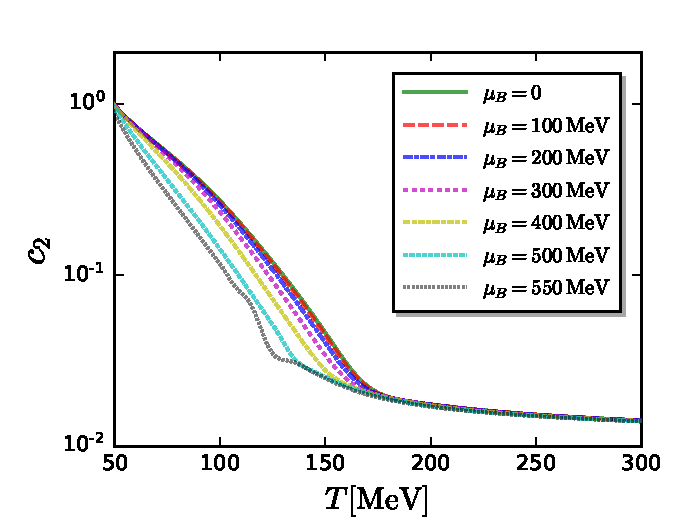
\includegraphics[width=0.45\textwidth]{c2}
\caption{Variance of temperature fluctuations as a function of the temperature with several different values of baryon chemical potential.}
\label{fig:c2}
\end{figure}
%%%%%%%%%%%%%%%%%%%%%%%%%%%%%
%

\textit{A new thermodynamic state function.} \label{sec:Wfunction}  We begin with a total derivative of the thermodynamic potential $\Omega$
\begin{align}
    \mathrm{d} \Omega=-S \mathrm{d} T-p \mathrm{d}V-N_B \mathrm{d} \mu_B\,, \label{eq:dOmega}
\end{align}
with the entropy $S$, temperature $T$, pressure $p$, volume $V$, baryon number $N_B$, and the baryon chemical potential $\mu_B$. Although we explicitly show $\mu_B$ as a representative of the conserved charge, Eq.~\labelcref{eq:dOmega} is readily generalized to include additional chemical potentials when other conserved charges are presented. The thermodynamic potential $\Omega$ is a state function of $T$, $V$ and $\mu_B$. By implementing a Legendre transformation upon $\Omega$ w.r.t. the conjugate pair $S$ and $T$, we introduce a new state function as
\begin{align}
    W=\Omega+TS\,. \label{eq:W-def}
\end{align}
One immediately recognizes that there is another relation for the state function $W$, that is,
\begin{align}
    W=U-\mu_B N_B\,,\label{}
\end{align}
resulting from the general thermodynamical relations, where $U$ denotes the energy. Inserting Eq.~\labelcref{eq:W-def} into Eq.~\labelcref{eq:dOmega}, one arrives at
\begin{align}
    \mathrm{d} W=T\mathrm{d} S-p \mathrm{d}V-N_B \mathrm{d} \mu_B\,, \label{eq:dW}
\end{align}
indicating that $W$ is a state function of $S$, $V$ and $\mu_B$.

In experimental measurements of mean transverse momentum fluctuations, finite acceptance cuts in the rapidity ($y$) and transverse momentum ($p_{T}$) range are applied, which signifies that the system volume and the chemical potential in Eq.~\labelcref{eq:dW} are approximately constant. While this approximation holds for high-energy collisions, we note that $\mu_B$ may vary in low-energy regions, e.g., fixed target collisions at RHIC, due to global baryon number conservation effects \cite{Braun-Munzinger:2020jbk, Vovchenko:2021kxx, Fu:2023lcm}. For the present study, we neglect these corrections and maintain the constant approximation. 

Recent measurements of mean transverse momentum fluctuations at RHIC and the LHC are performed at a fixed multiplicity of charged particles $N_{\mathrm{ch}}$, as shown in Ref. \cite{ALICE:2023tej,ATLAS:2024jvf,QM2025rutik,QM2025gao}. Since $N_{\mathrm{ch}}$ scales directly with the entropy of the system ($N_{\mathrm{ch}}\sim S$). Consequently, the state function $W$ in Eq.~\labelcref{eq:dW} becomes the appropriate thermodynamic potential for describing these experimental observables, as its natural variables directly correspond to the constrained quantities in the measures.

%
%%%%%%%%%%%%%%%%%%%%%%%%%%%%%
\begin{figure*}[t]
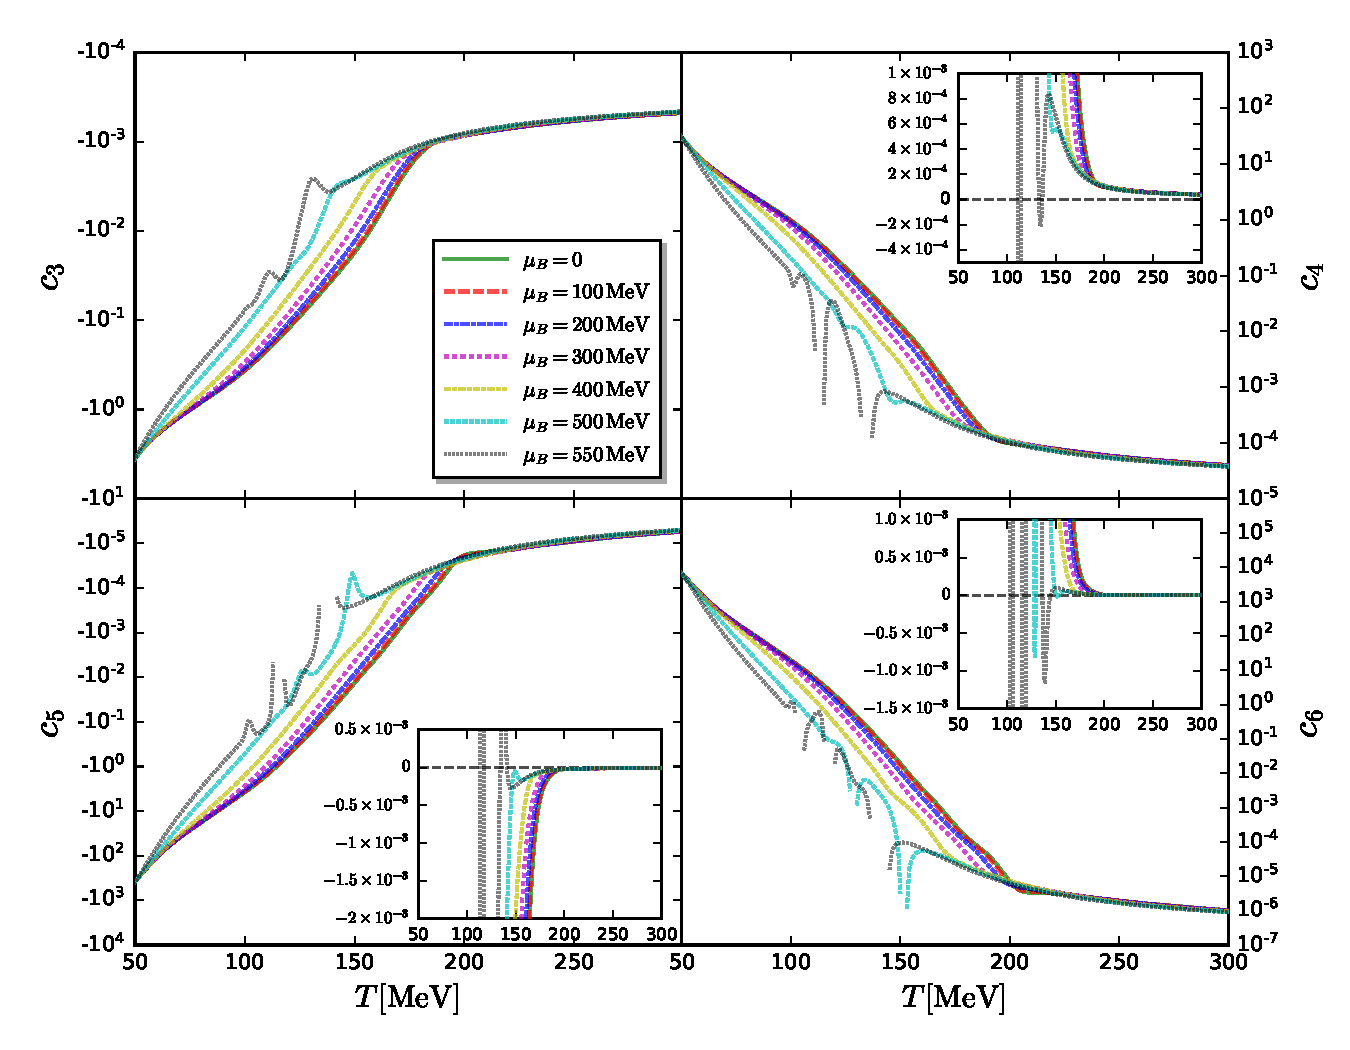
\includegraphics[width=0.8\textwidth]{c3toc6}
\caption{High-order temperature fluctuations of the third through sixth orders, i.e., $c_n$ in Eq.~\labelcref{eq:cn}, as functions of the temperature with several different values of baryon chemical potential. The insets show the respective plot by using the linear $y$-axis, where the zero-crossing is clear.}
\label{fig:c3-c6}
\end{figure*}
%%%%%%%%%%%%%%%%%%%%%%%%%%%%%
%

%
%%%%%%%%%%%%%%%%%%%%%%%%%%%%%
\begin{figure*}[t]
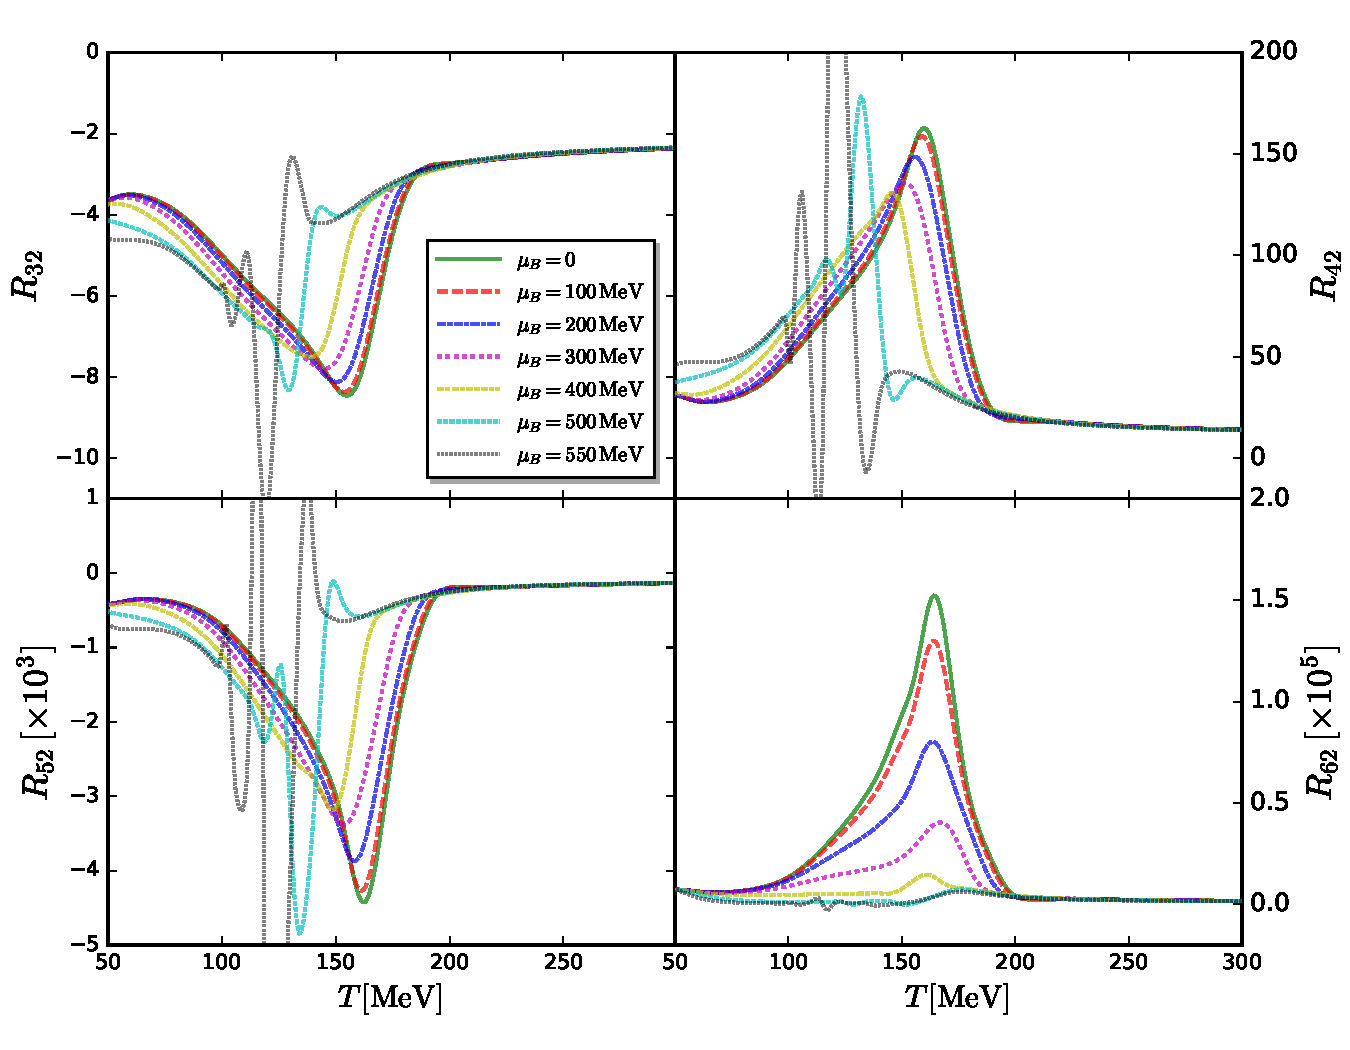
\includegraphics[width=0.8\textwidth]{Rmn}
\caption{Ratios between high-order temperature fluctuations and the variance, $R_{32}=c_3/c_2^2$, $R_{42}=c_4/c_2^3$, $R_{52}=c_5/c_2^4$, $R_{62}=c_6/c_2^5$, as functions of the temperature with several different values of baryon chemical potential.}
\label{fig:Rmn}
\end{figure*}
%%%%%%%%%%%%%%%%%%%%%%%%%%%%%
%


%%%%%%%%%%%%%%%%%%%%%%%%%%%%%%%%%%%%%%%%%%%%%%%%%%%
%%%%%%%%%%%%%%%%%%%%%%%%%%%%%%%%%%%%%%%%%%%%%%%%%%%

\textit{Temperature fluctuations derivations.} \label{sec:tem-fluc}  
Having established the relevance of the state function $W$ in Eq.~\labelcref{eq:dW} for heavy-ion collisions, we now derive the temperature fluctuations, or equivalently, the mean transverse momentum fluctuations of charged particles, computed from the derivative of $W$ w.r.t. $S$ for different orders.

For a fixed volume $V$, we define the intensive quantities:  the thermodynamic potential density $w=W/V$ and the entropy density $s=S/V$, one arrives at
\begin{align}
    w=-p+T s\,, \label{}
\end{align}
where $\Omega=-pV$ is used and the entropy density can be obtained from  $s=\frac{\partial p}{\partial T}$. The first-order derivative of $w$ w.r.t. $s$ produces the temperature
\begin{align}
    \frac{\partial w}{\partial s}=T\,. \label{}
\end{align}
Then, the $n$-th order fluctuation of temperature is obtained from the $n$-th order derivatives of $w$ w.r.t. $s$, to wit,
\begin{align}
    \langle(\Delta T)^n \rangle=T^{4n-4}\frac{\partial^n w}{\partial s^n}\,, \label{eq:DeltaTn}
\end{align}
with $\Delta T=T-\langle T \rangle$ and $n\geq 2$ ($n \in Z$), where $\langle \cdots \rangle$ denotes the ensemble average. It is convenient to adopt a dimensionless temperature fluctuation
\begin{align}
    c_n=\frac{\langle(\Delta T)^n \rangle}{T^n}\,. \label{eq:cn}
\end{align}
The cumulants $c_n$ can be expressed in terms of temperature derivatives of the pressure through fundamental thermodynamic relations. The first three nontrivial orders corresponding to the variance, skewness, and kurtosis of temperature fluctuations, are given by,
\begin{equation}\label{eq:c234}\begin{split}
    & c_2=T^2\left(\frac{\partial^2 p}{\partial T^2}\right)^{-1}\,\\[2ex]
    & c_3=-T^5\left(\frac{\partial^2 p}{\partial T^2}\right)^{-3}\frac{\partial^3 p}{\partial T^3}\,\\[2ex]
    & c_4=T^8\Bigg[3\left(\frac{\partial^2 p}{\partial T^2}\right)^{-5}\left(\frac{\partial^3 p}{\partial T^3}\right)^2-\left(\frac{\partial^2 p}{\partial T^2}\right)^{-4}\frac{\partial^4 p}{\partial T^4}\Bigg]\,.
\end{split} 
\end{equation}

This systematic approach can be extended to higher-order cumulants, e.g., the fifth and sixth hyper-order ones, which read
\begin{equation}\label{eq:c56}\begin{split}
    c_5=&T^{11}\Bigg[-15\left(\frac{\partial^2 p}{\partial T^2}\right)^{-7}\left(\frac{\partial^3 p}{\partial T^3}\right)^3-\left(\frac{\partial^2 p}{\partial T^2}\right)^{-5}\frac{\partial^5 p}{\partial T^5}\\[2ex]
    &+10\left(\frac{\partial^2 p}{\partial T^2}\right)^{-6}\frac{\partial^3 p}{\partial T^3}\frac{\partial^4 p}{\partial T^4}\Bigg]\,\\[2ex]
     c_6=&T^{14}\Bigg[105\left(\frac{\partial^2 p}{\partial T^2}\right)^{-9}\left(\frac{\partial^3 p}{\partial T^3}\right)^4-105\left(\frac{\partial^2 p}{\partial T^2}\right)^{-8}\\[2ex]
    &\times\left(\frac{\partial^3 p}{\partial T^3}\right)^2\frac{\partial^4 p}{\partial T^4}+10\left(\frac{\partial^2 p}{\partial T^2}\right)^{-7}\left(\frac{\partial^4 p}{\partial T^4}\right)^2\\[2ex]
    &+15\left(\frac{\partial^2 p}{\partial T^2}\right)^{-7}\frac{\partial^3 p}{\partial T^3}\frac{\partial^5 p}{\partial T^5}-\left(\frac{\partial^2 p}{\partial T^2}\right)^{-6}\frac{\partial^6 p}{\partial T^6}\Bigg]\,.
\end{split} 
\end{equation}

%%%%%%%%%%%%%%%%%%%%%%%%%%%%%%%%%%%%%%%%%%%%%%%%%%%
%%%%%%%%%%%%%%%%%%%%%%%%%%%%%%%%%%%%%%%%%%%%%%%%%%%

\textit{Numerical results.}\label{sec:numerical} We investigate QCD thermodynamics employing a 2+1 flavor LEFT within the fRG approach. As demonstrated in Ref. \cite{Wen:2018nkn}, this approach yields an equation of state (EoS) and baryon number fluctuations consistent with lattice QCD calculations. The setup of our LEFT is also recapitulated in the supplemental materials of this Letter.

To proceed, we systematically calculate the temperature derivatives of pressure: 
\begin{align}
    \chi_n=T^{n-4}\frac{\partial^n p}{\partial T^n}\,, \label{eq:chi}
\end{align}
which is dimensionless by means of normalization with appropriate powers of $T$. From the state function $\Omega$ in Eq.~\labelcref{eq:dOmega}, we identify the first and second order derivatives, $\chi_1$ and $\chi_2$, are just related to the entropy and heat capacity, respectively. Higher-order $\chi_n$ ($n \geq 2$) can be interpreted as entropy fluctuations of different orders. The numerical results of $\chi_n$ from the first to sixth orders calculated in the 2+1 flavor LEFT-fRG framework are presented in the supplement. We found that the entropy fluctuations increase and oscillate near the chiral crossover, and the strength and amplitude of the oscillation increase with the order of fluctuations or the value of baryon chemical potential. 

The temperature fluctuations in Eq.~\labelcref{eq:cn} can be reformulated in terms of $\chi_n$, defined in Eq.~\labelcref{eq:chi}. For the lowest-order cumulants, we obtain
\begin{align}
    c_2=&\frac{1}{\chi_2}\,, \qquad c_3=-\frac{\chi_3}{{\chi_2}^3}\,, \qquad c_4=3\frac{{\chi_3}^2}{{\chi_2}^5}-\frac{\chi_4}{{\chi_2}^4}\,. \label{}
\end{align}

The variance of temperature fluctuations, $c_2$, is inversely proportional to the variance of entropy fluctuations, i.e., the heat capacity $\chi_2$, as demonstrated in Fig.~\ref{fig:c2}. We observe that $c_2$ decreases with increasing temperature, reflecting the opposite trend of $\chi_2$ as shown in the supplement. This behavior indicates a significant suppression of temperature fluctuations in QGP phase compared to those in HRG phase. The suppression is more remarkable for high-order temperature fluctuations, as is evident in Fig.~\ref{fig:c3-c6} 
(note the logarithmic $y$-axis). A direct consequence of the suppression of temperature fluctuations at high temperature is that the distribution of temperature is wider in the region of lower temperature, that implies a negative skewness, as confirmed in the top-left panel of Fig.~\ref{fig:c3-c6}. While the kurtosis remains positive in most cases, its sign may reverse near the chiral crossover as it is sharpened continuously with the increase of baryon chemical potential. The sign change is more prominent for the hyper-order $c_5$ and $c_6$ cumulants.

In relativistic heavy-ion collisions, the event-averaged mean transverse momentum $\langle p_{T} \rangle$ of charged particles exhibits an approximate linear dependence on the system temperature, $\langle p_{T} \rangle = a\,T$ \cite{Gardim:2019xjs, Gardim:2019brr, Giacalone:2020lbm, Gardim:2024zvi}. The parameter $a$ represents the proportionality coefficient. In order to eliminate the influence from this coefficient that is not determined quite well, we instead analyze dimensionless ratios of temperature fluctuation cumulants: 
\begin{align}
    R_{32}=\frac{c_3}{c_2^2}\,, \quad R_{42}=\frac{c_4}{c_2^3}\,,\quad R_{52}=\frac{c_5}{c_2^4}\,,\quad R_{62}=\frac{c_6}{c_2^5}\,.\label{eq:R32R42}
\end{align}
where the powers of the variance in the denominators are chosen to balance the powers of $T$ as shown in Eqs.~\labelcref{eq:c234} and \labelcref{eq:c56}. The relevant ratios, presented in Fig.~\ref{fig:Rmn}, reveal that the cumulant ratios develop an increasingly rich nonmonotonic structure while exhibiting systematically reduced amplitudes with the increase of $\mu_B$, reflecting competing effects where enhanced critical fluctuations near the sharpened phase boundary emerge concurrently with the overall suppression of the magnitude of temperature fluctuation, as evidenced by the behavior shown in Figs.~\ref{fig:c2} and \ref{fig:c3-c6}. 



%%%%%%%%%%%%%%%%%%%%%%%%%%%%%%%%%%%%%%%%%%%%%%%%%%%
%%%%%%%%%%%%%%%%%%%%%%%%%%%%%%%%%%%%%%%%%%%%%%%%%%%
\textit{Conclusions.}\label{sec:conclusion} We have studied temperature fluctuations in hot QCD matter through a newly introduced thermodynamic state function that directly connects to mean transverse momentum fluctuations measured in heavy-ion collisions. Our approach yields analytic expressions for arbitrary-order temperature fluctuations, revealing their fundamental relationship with entropy, heat capacity, and high-order entropy fluctuations.  Implementing this in a 2+1 flavor LEFT-fRG framework, we firstly achieve obtaining numerical results that quantify the temperature fluctuations across different thermodynamic regimes.

As the system transitions from HRG to QGP phase with increasing temperature or the baryon chemical potential, the heat capacity of QCD matter increases substantially. This implies that a tiny change of the temperature would cost a huge amount of energy in the regime of high temperature. Therefore, the temperature tends not to change in comparison to the case in the regime of low temperature. In another word, the temperature fluctuations would be suppressed remarkably as the matter evolves from the HRG phase to the QGP phase with the increase of temperature or baryon chemical potential, as demonstrated in our calculations. The fact that temperature fluctuations at high temperature are smaller than those at low temperature leads to another direct consequence, that is, a negative skewness of temperature fluctuations. Such a signature emerges because the increasingly narrow fluctuation distribution at high temperature creates an asymmetric probability density weighted toward lower temperatures. In the future, temperature fluctuations represent a promising new observable for probing the QCD phase diagram in high baryon density regions, particularly through facilities at RHIC-BES, FAIR-CBM, NICA, and HIAF.



%%%%%%%%%%%%%%%%%%%%%%%%%%%%%%%%%%%%%%%%%%%%
\textit{Acknowledgements.} We thank Fei Gao,  Xuguang Huang, Jan M. Pawlowski for discussions and comments. W.J. Fu and S.Yin also would like to thank the members of the fQCD collaboration \cite{fQCD} for collaborations on related projects.
J.H. Chen\ is supported by the National Key Research and Development Program of China under Contract No. 2022YFA1604900, by the National Natural Science Foundation of China under Contract No. 12025501.
W.J. Fu\ is supported by the National Natural Science Foundation of China under Contract Nos.\ 12447102, 12175030. 
S. Yin\ is supported by the Alexander v.\ Humboldt Foundation. 
S. Yin\ acknowledges support by the Deutsche Forschungsgemeinschaft (DFG, German Research Foundation) through the CRC-TR 211 ``Strong-interaction matter under extreme conditions"– project number 315477589 – TRR 211.
C. Zhang\ is supported by the National Natural Science Foundation of China under Contract No. 12147101, by the Shanghai Pujiang Talents Program under Contract No. 24PJA009.

\bibliography{ref-lib}% 

\vfill 

%\vfill 

\end{document} 